Throughout all this document, we will use a lot of results from algebra. This
chapter is here to sum up these results and try to maintain the illusion that
this thesis is self-contained. Our references for standard results in algebra
are~\cite{Lang04} or~\cite{Perrin96}.
The reader familiar with the notions of finite
fields, algebraic function fields, or complexity model may very well skip this
chapter.
\minitoc

\begin{figure}
  \centering
  \begin{tikzpicture}[scale=0.8]
    \foreach \x in {0, 1,...,10} \coordinate (\x) at (32.7*\x:2);
    \draw[additive-structure] (0,0) circle (2);
    \draw[multiplicative-structure] (1) to [bend left] (2);
    \draw[multiplicative-structure] (2) to [bend left] (4);
    \draw[multiplicative-structure] (4) to [bend left] (8);
    \draw[multiplicative-structure] (8) to [bend right] (5);
    \draw[multiplicative-structure] (5) to [bend left] (10);
    \draw[multiplicative-structure] (10) to [bend right] (9);
    \draw[multiplicative-structure] (9) to [bend right] (7);
    \draw[multiplicative-structure] (7) to [bend right] (3);
    \draw[multiplicative-structure] (3) to [bend left] (6);
    \draw[multiplicative-structure] (6) to [bend right] (1);
    \foreach \x in {0, 1,...,10} \draw[fill] (32.7*\x:2) circle (.1);
    \foreach \x in {0, 1,...,10} \node (p) at (32.7*\x:2.4) {$\x$};
  \end{tikzpicture}
  \caption{Cyclic group structure of $(\mathbb{F}_{11}, +)$ (red) and
  $(\mathbb{F}_{11}^\times, \times)$ (blue).}
  \label{fig:finite-field}
\end{figure}
 
\clearpage
\section{Finite fields}

Finite fields are ubiquitous in cryptography and coding theory, probably because
their field structure, a rigid one, allows to understand how they work, and
their finiteness makes them easier to represent on a computer. They are also
everywhere in this thesis, and are probably on almost every paper I
wrote on during these last three years. They are quite important. A detailed
book about finite fields is~\cite{LN97}.

\subsection{Finite field structure}

A \emph{finite field} is a field $\K$ whose cardinality is finite. The first
examples of finite fields are the rings 
\[
  \mathbb{Z}/p\mathbb{Z}
\]
with $p\in\mathbb{N}$ a prime number. More generally, we denote by
$\mathbb{F}_{q}$ the finite field with $q$ elements. The cardinality of a finite
field is very well understood.
\begin{prop}
 There exists a unique (up to isomorphism) finite field of cardinality $q = p^l$
 for each prime number $p\in\mathbb{N}$ and integer $l\geq1$, and every finite
 field has cardinality of the form $q = p^l$.
\end{prop}
Let $q=p^l$ a prime power, there are several ways of representing
\emph{the} finite field with $q$ elements, but the one that we will almost
always have in mind is the following.

\begin{prop}
Let $P\in\mathbb{F}_p[x]$ be an
irreducible polynomial of degree $l$ with coefficients in $\mathbb{F}_p$. Then
\[
  \mathbb{F}_p[x]/(P(x))
\]
is a finite field with $q = p^l$ elements.
\end{prop}
We often write
\[
  \mathbb{F}_q \cong \mathbb{F}_{p}[x]/(P(x))\cong \mathbb{F}_p(\alpha)
\]
in order to say that we work with a finite field of $q$ elements, represented by
the quotient $\mathbb{F}_{p}[x]/(P(X))$, and where the projection of $x$ in the
quotient is denoted by $\alpha=\bar x$.

\subsection{Subfields and field extensions}

The finite field $\mathbb{F}_{p^l}$ is a
field extension of $\mathbb{F}_{p}$ of dimension $l$, \ie it is a
$\mathbb{F}_{p}$-vector space of dimension $l$. When dealing with the vector
space structure of $\mathbb{F}_{p^l}=\mathbb{F}_{p}(\alpha)$, we almost always choose to work with the
canonical basis 
\[
  1, \alpha, \alpha^2, \dots, \alpha^{l-1}.
\]
Other interesting types of bases exist, such as for example normal
bases~\cite{Gao93}, but we always specify the basis when it is not clear from
the context.
Given $q=p^m$ a prime power and
$l\in\mathbb{N}$ an integer, we also write 
\[
  \mathbb{F}_{q^l}
\]
the field with $q^l = p^{ml}$ elements. We have
\[
  \mathbb{F}_{q^l}\cong\mathbb{F}_{p^{lm}},
\]
but the difference is that we see $\mathbb{F}_{q^l}$ as an extension of
$\mathbb{F}_{q}$ of dimension $l$, and not as an extension of the prime field
$\mathbb{F}_p$. Again, we usually think that our field $\mathbb{F}_{q^l}$ is
represented as
\[
  \mathbb{F}_{q^l}=\mathbb{F}_q[x]/(P(x)),
\]
where $P(x)\in\mathbb{F}_{q}[x]$ is an irreducible polynomial of degree $l$ with
coefficients in the base field $\mathbb{F}_q$. The subfields of
$\mathbb{F}_{q^l}$ are also well understood.
\begin{prop}
  \label{prop:subfields}
  Let $q=p^m$ be a prime power and $l\in\mathbb{N}$ an integer. Then there is
  an extension $\mathbb{F}_{q^m}$ of $\mathbb{F}_q$ of degree $m$ 
  included in $\mathbb{F}_{q^l}$
  \[
    \mathbb{F}_{q^m}\subset\mathbb{F}_{q^l}
  \]
  if and only if $m$ divides
  $l$. The elements in this subfield of $\mathbb{F}_{q^l}$ are the roots of the
  polynomial
  \[
    x^{q^m}-x
  \]
  in $\mathbb{F}_{q^l}$.
\end{prop}
Figure~\ref{fig:F12} describes the subfields of $\mathbb{F}_{q^{12}}$, as an
illustration of Proposition~\ref{prop:subfields}.
\begin{figure}
  \centering
  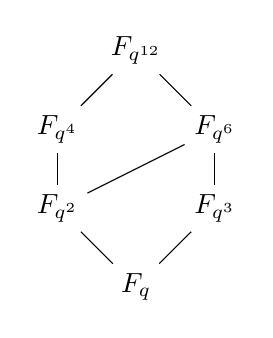
\begin{tikzpicture}
    \node (1) at (0,0) {$\mathbb{F}_{q}$}; 
    \node (2) at (-1,1) {$\mathbb{F}_{q^2}$}; 
    \node (3) at (1,1) {$\mathbb{F}_{q^3}$}; 
    \node (4) at (-1,2) {$\mathbb{F}_{q^4}$}; 
    \node (6) at (1,2) {$\mathbb{F}_{q^6}$}; 
    \node (12) at (0,3) {$\mathbb{F}_{q^{12}}$}; 
    \draw (1) -- (2);
    \draw (1) -- (3);
    \draw (2) -- (4);
    \draw (2) -- (6);
    \draw (3) -- (6);
    \draw (6) -- (12);
    \draw (4) -- (12);
  \end{tikzpicture}
  \caption{The subfields of $\mathbb{F}_{q^{12}}$. Two fields are linked if one is a
subfield of the other.}
  \label{fig:F12}
\end{figure}
The $\mathbb{F}_q$-automorphisms of the extension $\mathbb{F}_{q^l}$ are given
by the following result.
\begin{prop}
  Let $q=p^m$ be a prime power and $l\in\mathbb{N}$ an integer.
  The group of $\mathbb{F}_q$-automorphisms of $\mathbb{F}_{q^l}$ is a cyclic
  group of order $l$ generated by
  \[
    \sigma : t\mapsto t^q.
  \]  
\end{prop}
Let $u\in\mathbb{F}_{q^l}$, the conjugates of $u$ are the elements
\[
  \sigma(u), \sigma^2(u), \dots, \sigma^{l-1}(u)
\]
and the orbit of $u$ is the set
\[
  \left\{ u, \sigma(u), \dots, \sigma^{l-1} \right\}.
\]
This orbit might have any length $m$ dividing $l$. The orbit of $u$ is of length
exactly $m$ if and only if the smallest subfield $u$ belongs to is the subfield
$\mathbb{F}_{q^m}$ of $\mathbb{F}_{q^l}$. We also sometimes write
\[
  u^\sigma = \sigma(u).
\]
Two maps, defined with the conjugates of a given element,
will play a very important role, the \emph{trace} and the \emph{norm}.
\begin{defi}[Trace and norm]
  Let $q$ a prime power and 
  \[
    \mathbb{F}_{q^l}/\mathbb{F}_q
  \]
  an extension of degree $l$, let $G$ be the group of
  $\mathbb{F}_q$-automorphisms of $\mathbb{F}_{q^l}$, and let
  $u\in\mathbb{F}_{q^l}$. Then the \emph{trace} of $u$ is
  \[
    \tr_{\mathbb{F}_{q^l}/\mathbb{F}_q}(u) = \sum_{\sigma\in G}u^\sigma
  \]
  and the \emph{norm} of $u$ is
  \[
    N_{\mathbb{F}_{q^l}/\mathbb{F}_q}(u)=\prod_{\sigma\in G}u^\sigma.
  \]
\end{defi}
We may only write $\tr$ or $N$ when the extension considered is clear from the
context. The trace over the field $\mathbb{F}_{q}$ is a $\mathbb{F}_{q}$-linear
map, and the norm is a multiplicative map, they are also both \emph{transitive},
as described in the next proposition.
\begin{prop}
  Let $q\in\mathbb{N}$ a prime power and $a\,|\,b\,|\,c$ three integers, giving
  the tower of extensions that follows.
  \begin{center}
  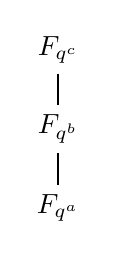
\begin{tikzpicture}
    \node (a) at (0,0) {$\mathbb{F}_{q^a}$}; 
    \node (b) at (0,1) {$\mathbb{F}_{q^b}$}; 
    \node (c) at (0,2) {$\mathbb{F}_{q^c}$}; 
    \draw (a) -- (b);
    \draw (b) -- (c);
  \end{tikzpicture}
  \end{center}
  Let $u\in\mathbb{F}_{q^c}$, then
  \[
    \tr_{\mathbb{F}_{q^c}/\mathbb{F}_{q^a}}(u) =
    \tr_{\mathbb{F}_{q^b}/\mathbb{F}_{q^a}}(\tr_{\mathbb{F}_{q^c}/\mathbb{F}_{q^b}}(u))
  \]
  and
  \[
    N_{\mathbb{F}_{q^c}/\mathbb{F}_{q^a}}(u) =
    N_{\mathbb{F}_{q^b}/\mathbb{F}_{q^a}}(N_{\mathbb{F}_{q^c}/\mathbb{F}_{q^b}}(u)).
  \]
\end{prop}
Finally, the map
\[
  (x, y)\mapsto\tr(xy)
\]
is a non-degenerate bilinear map that we will also sometimes write as
\[
  \ps{x}{y} = \tr(xy).
\]
%
%\subsection{Kummer extensions}
%
%Kummer extensions are a particular kind of extension, they play a special role in
%our construction of lattices of extension presented in
%Chapter~\ref{chap:lattice}. We follow the presentation of~\cite{Lang04}.

\section{Algebraic function fields}
\label{sec:algebraic-function-fields}

% Contents
% ========
%
% - algebraic function field
% - place
% - degree of a place
% - divisor
% - big theorems
% - definition of the genus ?

Together with algebraic curves, algebraic function fields are a way of
describing the algorithms of Chapters~\ref{chap:bilinear}
and~\ref{chap:hypersymmetric}. In this document, we choose to use the algebraic
function field point of view. The function fields we need are constructed
on top of finite fields, so we present the theory with that context in mind. For
this section, our reference is~\cite{Stichtenoth09}. In all the section, $\K$ is
a finite field of characteristic $p$.

\subsection{Places}

Let us first define what an algebraic function field is, together with important
notions leading to the definition of \emph{places}.
\begin{defi}[Algebraic function field]
  An \emph{algebraic function field} $F$ of one variable over $\K$ is an
  extension field 
  \[
    F/\K
  \]
  such that $F$ is a finite algebraic extension of
  $\K(x)$ for some element $x\in F$ which is transcendental over $\K$.
\end{defi}
From now on, the notation $F$ will represent an algebraic function field over
$\K$. Since it is not critical to the theory, we also assume that $\K$ is
algebraically closed in $\K$ for simplicity.

\begin{defi}[Valuation ring]
  A \emph{valuation ring} $\vr$ of the function field $F/\K$ is a ring 
  \[
    \vr \subset F
  \]
  with the following properties
  \begin{enumerate}
    \item $\K\subsetneq\vr\subsetneq F$;
    \item for all $z\in F$, we have $z\in\vr$ or $z^{-1}\in\vr$.
  \end{enumerate}
\end{defi}
\begin{prop}
  \label{prop:valring}
Let $\vr$ be the a valuation ring of the function field $F$. 
\begin{enumerate}[(a)]
    \item The ring $\vr$ is local, \ie it has a unique maximal ideal that is given
      by
      \[
        P = \vr\setminus\vr^\times
      \]
      where $\vr^\times$ is the group of units of the ring $\vr$.
    \item \label{cond:valring} For any nonzero $x\in F$, we have
      \[
        x\in P\Longleftrightarrow x^{-1}\notin\vr.
      \]
\end{enumerate}
\end{prop}
\begin{thm}
  \label{thm:discrete-valring}
 Let $\vr$ be the valuation ring of the function field $F$ and $P$ be its unique
 maximal ideal. Then
 \begin{enumerate}[(a)]
   \item The ideal $P$ is principal.
   \item If $P=t\vr$ then any nonzero $z\in F$ has a unique representation of
     the form
     \[
       z = t^n u
     \]
     with $n\in\mathbb{Z}$ and $u\in\vr^\times$
   \item The ring $\vr$ is a principal ideal domain. More precisely, if $P=t\vr$
     and
     \[
       \left\{ 0 \right\}\neq I\subseteq\vr
     \]
     is an ideal then
     \[
       I = t^n\vr
     \]
     for some $n\in\mathbb{N}$.
 \end{enumerate}
\end{thm}
A ring having the properties described in Theorem~\ref{thm:discrete-valring} is
called a \emph{discrete valuation ring}.
\begin{defi}[Place]
  A \emph{place} $P$ of $F$ is the maximal ideal of some valuation ring $\vr$ of $F$.
\end{defi}
\begin{defi}[Prime element]
  Let $\vr$ be a valuation ring and $P$ its maximal ideal. Any element $t\in P$
  such that
  \[
    P = t\vr
  \]
  is called a \emph{prime element} for $P$. It is also sometimes called a
  \emph{local parameter} or a \emph{uniformizing variable}.
\end{defi}
If $\vr$ is a valuation ring of $F$ and if $P$ is its maximal ideal, then $\vr$
is uniquely determined by $P$, indeed we have
\[
  \vr = \left\{ z\in F\mid z^{-1}\notin P \right\}
\]
thanks to Proposition~\ref{prop:valring}\ref{cond:valring}. Thus, the notions of
valuation rings and places are essentially equivalent. There is a third way of
describing a place, given by discrete valuations.
\begin{defi}[Discrete valuation]
  A \emph{discrete valuation} of $F$ is a function
  \[
    v:F\to\mathbb{Z}\cup\left\{ \infty \right\}
  \]
  with the following properties:
  \begin{enumerate}
    \item $v(x) = \infty \Leftrightarrow x=0$;
    \item for any $x,y\in F$, $v(xy) = v(x)+v(y)$;
    \item for any $x,y\in F$, $v(x+y)\geq\min(v(x), v(y))$;
    \item there exists an element $z\in F$ with $v(z)=1$;
    \item for any nonzero element $a\in\K$, $v(a) = 0$.
  \end{enumerate}
\end{defi}
Here, the symbol $\infty$ means an element that is not in $\mathbb{Z}$, such
that $\infty+\infty = \infty + n = \infty$ and $\infty > m$ for any
$m,n\in\mathbb{Z}$.
\begin{defi}
  To any place $P\in\mathbb{P}_F$, we associate a function
  \[
    v_P:F\to\mathbb{Z}\cup\left\{ \infty \right\}
  \]
  that is in fact a discrete valuation ring. Let $t$ be a prime element for $P$.
  Then every nonzero element $z\in F$ has a unique representation
  \[
    z = t^n u
  \]
  with $u\in\vr^\times$ and $n\in\mathbb{Z}$. We define
  \[
    v_P(z)\eqdef n
  \]
  and
  \[
    v_P(0)\eqdef\infty.
  \]
\end{defi}
This definition does not depend on the prime element $t$ that was chosen. It
allows us to give the third equivalent way of describing a place of $F$.
\begin{thm}
 Let $F$ be a function field.
 \begin{enumerate}[(a)]
   \item For any place $P\in\mathbb{P}_F$, the function $v_P$ defined above is a
     discrete valuation of $F$. Moreover, we have
     \begin{align*}
       \vr_P &= \left\{ z\in F\mid v_P(z)\geq0 \right\},\\
       \vr_P^\times &= \left\{ z\in F\mid v_P(z)>0 \right\},\\
       P &= \left\{ z\in F\mid v_P(z)=0 \right\}.
     \end{align*}
     An element $x\in F$ is a prime element for $P$ if and only if $v_P(x)=1$.
   \item Conversely, if $v$ is a discrete valuation of $F$, then the set
     \[
       P = \left\{ z\in F\mid v(z)>0 \right\}
     \]
     is a place of $F$, and
     \[
       \vr_P = \left\{ z\in F\mid v(z)\geq0\right\}
     \]
     is the corresponding valuation ring.
 \end{enumerate}
\end{thm}
We let $\mathbb{P}_F$ be the set of places of $F$. If $P\in\mathbb{P}_F$ is a
place of $F$, we denote by $\vr_P$ the corresponding valuation ring. Since $P$
is a maximal ideal of $\vr$, we also know that the quotient ring
\[
  F_P = \vr_P/P
\]
is a field. We call this field $F_P$ the \emph{residue class field} of $P$.
\begin{defi}[Residue class map]
Let $P\in\mathbb{P}_F$ be a place of $F$. For $x\in F$, we let 
\[
  x(P)
\]
be the residue class of $x$ modulo $P$. If $x\notin \mathcal O_P$, we define $x(P)=\infty$.
The map from $F$ to $F_P\cup\left\{ \infty \right\}$
\[
  x\mapsto x(P)
\]
is called the \emph{residue class map}.
\end{defi}
\begin{defi}[Degree of a place]
  Let $P\in\mathbb{P}_F$ be a place of $F$. The residue class field $F_P$ is a
  finite extension of $\K$ and we call
  \[
    \deg P = \left[ F_P\,:\,\K \right]
  \]
  the \emph{degree} of $P$.
\end{defi}
In fact, the degree of a place if always finite. If $P$ is a place of degree
$1$, then its residue class field $F_P$ is equal to
\[
  F_P = \K.
\]
The residue class map then maps $F$ to $\K\cup\left\{ \infty \right\}$. In
particular, if $\K$ is algebraically closed, any place has degree $1$, thus we
can interpret an element $z\in F$ as a function
\[
  \begin{array}{cccc}
    z:&\mathbb{P}_F&\to&\K\cup\left\{ \infty \right\}\\
    & P & \mapsto & z(P)
  \end{array}.
\]
This justifies the name \emph{function field} for $F$. With this interpretation,
places of degree $1$ are viewed as points and elements in $\K$ are viewed as
constant functions. This is also a reason behing the following terminology.
\begin{defi}[Zero and pole]
  Let $z\in F$ be an element in the function field $F$ and $P\in\mathbb{P}_F$ a
  place of $F$. We say that $P$ is a \emph{zero} of $z$ if $v_P(z)>0$ and that
  $P$ is a \emph{pole} of $z$ if $v_P(z)<0$. If $v_P(z) = n > 0$, then $P$ is a
  \emph{zero of order} $n$; if $v_P(z) = -n < 0$, then $P$ is a \emph{pole of
  order} $n$.
\end{defi}
Note that if $P$ is a zero of $z\in F$, we have $z(P) = 0$, while we have
$z(P)=\infty$ if $P$ is a pole of $z$. Another important result states that
every element not in $\K$ yields a non-constant function.
\begin{prop}
 Let $F$ be a function field and $z\in F$ an element in $F$ that is
 not in $\K$. Then $z$ has at least one zero and one pole. In particular, this
 proves that the set $\mathbb{P}_F$ of places is not empty.
\end{prop}

\subsection{Independence of valuations}

Before talking about the central notions of divisors and Riemann-Roch spaces, we
must mention one important theorem called the \emph{weak approximation theorem}
(also refered to as \emph{theorem of independence}). It essentially says that
if we have pairwise distinct discrete valuations $v_1, \dots, v_n$ of $F$ and an
element $z\in F$ for which we know the values $v_1(z), \dots, v_{n-1}(z)$, then
we cannot conclude anything about the value $v_n(z)$.
\begin{thm}
  \label{thm:weak-approx}
  Let $F$ be a function field, $P_1, \dots, P_n\in\mathbb{P}_F$ be pairwise
  distinct places of $F$, $x_1, \dots, x_n\in F$ be elements in $F$ and $r_1,
  \dots, r_n\in\mathbb{Z}$ be integers. Then there is some $x\in F$ such that
  \[
    v_{P_i}(x-x_i) = r_i\text{ for all }1\leq i\leq n.
  \]
\end{thm}
The name ``approximation theorem'' comes from the fact that $v_{P_i}(x-x_i)$ can
be interpreted as some ``distance'' between $x$ and $x_i$. With this
interpretation, Theorem~\ref{thm:weak-approx} says that the distances between
$x$ and $x_i$ can be made simultaneously arbitrarily small using \emph{one}
element $x$. This theorem allows us to mention important results.
\begin{cor}
  Any function field $F$ has infinitely many places.
\end{cor}
\begin{prop}
  Let $F$ be a function field and $P_1, \dots, P_r$ be the zeros of some element
  $x\in F$. Then
  \[
    \sum_{i=1}^r{v_{P_i}(x)\cdot\deg P_i}\leq \left[ F:\K(x) \right].
  \]
\end{prop}
\begin{cor}
  In a function field $F$, any nonzero element $x\in F$ has only finitely many
  zeros and poles.
\end{cor}

\subsection{Divisors}

Now that we know what places are, we can define divisors. In this section, we
keep the notation of the last section: we let $F$ be an algebraic function field
over a finite field $\K$ of characteristic $p$.
\begin{defi}[Divisor]
  The \emph{divisor group} $\Div(F)$ of $F$ is defined as the free abelian group generated
  with the places of $F$. The elements of $\Div(F)$ are called the
  \emph{divisors} of $F$. In other words, a divisor is a formal sum
  \[
    D = \sum_{P\in\mathbb{P}_F} n_P\cdot P
  \]
  with $n_P\in\mathbb{Z}$ and $n_P=0$ for all but finitely many places $P$.
\end{defi}
\begin{defi}[Support]
  Let 
  \[
    D = \sum_{P\in\mathbb{P}_F} n_P\cdot P
  \]
  be a divisor of $F$. We define the \emph{support} of $D$ as
  \[
    \supp D = \left\{ P\in\mathbb{P}_F\,|\,n_P\neq 0 \right\}.
  \]
\end{defi}
Two divisors 
\[
  D = \sum_{P\in\mathbb{P}_F} n_P\cdot P
\]
and
\[
  D' = \sum_{P\in\mathbb{P}_F} n_P'\cdot P
\]
in $\Div(F)$ are added coefficient-wise:
\[
  D+D' = \sum_{P\in\mathbb{P}_F} (n_P+n_P')\cdot P
\]
and the zero element is the divisor
\[
  0 \eqdef \sum_{P\in\mathbb{P}_F} n_P\cdot P
\]
with $n_P=0$ for all places $P\in\mathbb{P}_F$. If
\[
  D = \sum_{P\in\mathbb{P}_F}n_P\cdot P
\]
is a divisor $\Div(F)$ and $Q\in\mathbb{P}_F$ is a place of $F$, we let 
\[
  v_Q(D) = n_Q
\]
be the coefficient multiplying $Q$ in the formal sum $D$. We then have
\[
  \supp D = \left\{ P\in\mathbb{P}_F\mid v_P(D)\neq 0 \right\}.
\]
We then define a partial ordering on $\Div(F)$ by
\[
  D_1 \leq D_2 \overset{\text{def}}{\Longleftrightarrow} v_P(D_1)\leq v_P(D_2)\text{ for all
  }P\in\mathbb{P}_F.
\]
A divisor $D\geq 0$ is called \emph{positive} (or \emph{effective}).
\begin{defi}[Degree]
  Let $D\in\Div(F)$ be a divisor, its \emph{degree} is defined by
  \[
    \deg(D) = \sum_{P\in\mathbb{P}_F}v_P(D)\deg(P)
  \]
  and yields a homomorphism $\deg:\Div(F)\to\mathbb{Z}$.
\end{defi}
\begin{defi}
  Let $x\in F$ be a nonzero element in $F$, $Z\subset\mathbb{P}_F$ be the set of
  its zeros and $N\subset\mathbb{P}_F$ be the set of its poles. Then, we define
  \begin{align*}
    (x)_0 &= \sum_{P\in Z}v_P(x)P ,\,\text{ the \emph{zero divisor} of }x,\\
    (x)_\infty &= \sum_{P\in N}(-v_P(x))P ,\,\text{ the \emph{pole divisor} of
  }x,\\
    (x) &= (x)_0 - (x)_\infty ,\,\text{ the \emph{principal divisor} of }x.
  \end{align*}
\end{defi}
We have $(x)_0\geq0, (x)_\infty\geq0$ and
\[
  (x) = \sum_{P\in\mathbb{P}_F}v_P(x)P.
\]
If $x\in K$, then $x$ does not have zeros nor poles and the sum is then empty,
conversely a function in $F\setminus\K$ has at least one zero and one pole, we
thus have
\[
  x\in\K\Leftrightarrow (x)=0.
\]
\begin{defi}[Equivalence]
  Let $D, D'\in\Div(F)$ be two divisors of $F$. We can define an equivalence
  relation by
  \[
    D\sim D'\Longleftrightarrow\text{ there exists }x\in F\text{ such that }D =
    D'+(x).
  \]
  In that case, we say that $D$ and $D'$ are \emph{linearly equivalent}, or just
  \emph{equivalent}.
\end{defi}
Principal divisors play a crucial role in the algebraic function field theory.
They allow us to define spaces that play a fundamental role.
\begin{defi}
  Let $D\in\Div(F)$ be a divisor of $F$. We let
  \[
    L(D) = \left\{ x\in F\mid(x)\geq -D \right\}\cup\left\{ 0 \right\}.
  \]
\end{defi}
This definition can be interpreted in the following way: if
\[
  D = \sum_{i=1}^rn_iP_i - \sum_{j=1}^sm_jQ_j,
\]
with $n_i>0$ and $m_j>0$, then $L(D)$ consists of all elements $x\in F$ such
that
\begin{enumerate}
  \item for all $1\leq j\leq s$, $x$ has a zero of order at least $m_j$ at $Q_j$;
  \item the places $P_1, \dots, P_r$ are the only poles of $x$, and for all
    $1\leq i\leq r$, the order of the pole $P_i$ is bounded by $n_i$.
\end{enumerate}
We recall some properties of the spaces $L(D)$ in
Proposition~\ref{prop:LD-spaces}.
\begin{prop}
  \label{prop:LD-spaces}
 Let $D\in\Div(F)$ be a divisor.
 \begin{enumerate}[(a)]
   \item $L(D)$ is a finite-dimensionnal $\K$-vector space.
   \item $L(D)\neq\left\{ 0 \right\}$ if and only if there exists a divisor
     $D'\sim D$ with $D'\geq0$.
   \item If $D'\sim D$, then $L(D)$ and $L(D')$ are isomorphic as $\K$-vector
     spaces.
   \item $x\in L(D)$ if and only if $v_P(x)\geq - v_P(D)$ for all
     $P\in\mathbb{P}_F$.
   \item $L(0)=\K$.
   \item If $\deg(D)<0$ then $L(D)=\left\{ 0 \right\}$. In particular if $D<0$
     then $L(D)=\left\{ 0 \right\}$.
 \end{enumerate}
\end{prop}
\begin{defi}[Dimension]
  Let $D\in\Div(F)$ be a divisor of $F$. The \emph{dimension} of $D$ is denoted
  by $\ell(D)$ and is defined by
  \[
    \ell(D) = \dim L(D).
  \]
\end{defi}
We can now define the most important invariant of a function field $F$, its
\emph{genus}.
\begin{defi}[Genus]
  Let $F$ be a function field. The \emph{genus} $g$ of $F$ is the nonnegative
  integer defined by
  \[
    g = \max\left\{ \deg D-\ell(D)+1\mid D\in\Div(F) \right\}.
  \]
\end{defi}
\begin{defi}[Index of specialty]
  \label{defi:index-specialty}
  Let $D\in\Div(F)$ be a divisor of $F$, the nonnegative integer
  \[
    i(D) = \ell(D) - \deg(D) + g - 1
  \]
  is called the \emph{index of specialty} of $D$. A divisor $D$ such that
  $i(D)=0$ is called \emph{non-special}; a divisor $D$ such that $i(D)>0$ is
  called \emph{special}.
\end{defi}
\begin{defi}[Canonical divisor]
  Let $F$ be a function field of genus $g$. A divisor $W$ of degree $\deg W = 2g-2$ and
  dimension $\ell(W) = g$ is called a \emph{canonical divisor}.
\end{defi}
In fact, all canonical divisors are equivalent, and they are involved in the
very important Riemman-Roch theorem.
\begin{thm}[Riemann-Roch]
  \label{thm:riemann-roch}
  Let $W\in\Div(F)$ be a canonical divisor of $F$. Then, for any divisor
  $D\in\Div(F)$, we have
  \[
    \ell(D) = \deg(D) + 1 - g + \ell(W-D).
  \]
\end{thm}
\begin{rem}
Note that with Definition~\ref{defi:index-specialty},
Theorem~\ref{thm:riemann-roch} means that
\[
  i(D) = \ell(W-D).
\]
\end{rem}

\section{Complexity models}
\label{sec:complexity-models}

When studying algorithms, it is of central interest to understand how our algorithms
\emph{scale}, \ie to understand how they perform if the size of the input is
getting larger and larger. Complexity theory studies this phenomenon and gives us models
of computation in order to quantify the behaviour of our algorithms. Depending
on the situation, not all models are relevant, and one has to balance between
the concreteness of a model and its ease of use. An extreme viewpoint is to
specify an operating system with a compiled programming language and to compare
the running time or the memory requirements between algorithms. The advantage of
such a model is that it is very concrete, but it is also its main disadvantage
because it makes the model hard to use. Thus, there exist other models of
\emph{idealized} computers, such as Turing machines~\cite{Papadimitriou03},
random access machines, or the algebraic complexity model.
We use the latter, that we present in more details in the next section.

\subsection{Algebraic complexity}
\label{sec:algebraic-complexity}

This model is widely presented in~\cite{BCS13}, we only give a brief
presentation of the subject. This model assumes that we use an abstract computer
that is able to perform operations in some base field $\K$ at a constant, unit
cost. We also assume that accessing the memory of the computer is free.
Algebraic complexity is especially useful with algorithms dealing with
algebraic structures. This is very handy for us, since
we usually work with algebras
\[
  (\A, +, \times, \cdot)
\]
over some base field $\K$. As an example, with this model, the complexity of an
addition in the extension field
\[
  \mathbb{F}_4 = \mathbb{F}_2[T]/(T^2+T+1) = \mathbb{F}_2(x)
\]
where $x=\bar T$, if elements are represented in the basis $\left\{ 1, x
\right\}$, is $2$, because we only need $2$ additions in $\mathbb{F}_2$ to
perform an addition in $\mathbb{F}_4$. Indeed, if
\[
  a = a_0 + a_1x\in\mathbb{F}_4
\]
and
\[
  b = b_0 + b_1x\in\mathbb{F}_4,
\]
we have
\[
  a+b = (a_0+b_0)+(a_1+b_1)x.
\]
In the case of a multiplication, we have
\[
  ab = (a_0b_0+a_1b_1) + (a_0b_1+a_1b_0)x,
\]
so the complexity of a multiplication in $\mathbb{F}_4$ (at least with this
formula) is $6$, because we need
$4$ multiplications and $2$ additions in $\mathbb{F}_2$. In the context of
finite fields, it makes sense to consider that the cost of an operation is
independent of the operands, because the elements have a fixed size; but this is
no longer the case in other rings, for example in $\mathbb{Z}$, $\mathbb{Q}$,
$\mathbb{R}$, or $\mathbb{C}$. We could also argue that the different operations
in $\K$ should not have the same cost, we thus present an other manner of
computing the complexity of an algorithm, that is called \emph{bilinear
complexity}, in Chapter~\ref{chap:bilinear}.

\subsection{Landau notations}

In order to describe the asymptotic behaviour of an algorithm, we use the
classical \emph{big O} and \emph{little o} notations $O$ and $o$. Let $f:\mathbb{R}\to\mathbb{R}$ and
$g:\mathbb{R}\to\mathbb{R}$ be two functions, we write
\[
  f(x) = O(g(x))
\]
if there exist $M\in\mathbb{R}$ and $C>0$ such that
\[
  \forall x\geq M,\,|f(x)|\leq Cg(x).
\]
and we write
\[
  f(x)=o(g(x))
\]
if there exist $M\in\mathbb{R}$ and $\varepsilon:\mathbb{R}\to\mathbb{R}$, a
function with $\varepsilon(x)\to 0$ when $x\to\infty$, such
that
\[
  \forall x\geq M,\,|f(x)|\leq \varepsilon(x)g(x).
\]
We say that $f$ is equivalent to $g$ and we write
\[
  f(x)\sim g(x)
\]
if 
\[
 f(x)-g(x) = o(g(x))
\]
when $x\to\infty$. Finally, we also use the \emph{soft O} notation $\tilde{O}$ to neglect
logarithmic factors in the big O notation, we write
\[
  f(x) = \tilde{O}(g(x))
\]
if there exist some $k$ with $f(x) = O(g(x)\log^k(g(x)))$.

\section{Foundamental algorithms}
\label{sec:foundamental-algos}

In this section, we briefly review the fundamental algorithms that are used in
the thesis. Unless explicitely stated otherwise, we measure the complexities
using the algebraic complexity presented in
Section~\ref{sec:algebraic-complexity}, \ie in number of operations $+, \times,
\div$ in some base field $\K$. References for this section are~\cite{GG13,
BCGLLSS17, BDDFS17}.

\subsection{Finite field arithmetic}

Since finite fields are so important in this thesis, we first review the
complexity of the basic operations in finite fields. We let
\[
  \K = \mathbb{F}_q
\]
be the finite field with $q$ elements, where $q$ is a prime power and we let $p$
be the characteristic of $\K$. We consider $\mathbb{F}_{q^n}$ a finite field
extension of degree $n$ of $\K$, and we assume that the elements in
$\mathbb{F}_{q^n}$ are represented by univariate polynomials in $\K\left[ x
\right]$. We let $P\in\K\left[ x \right]$ be the irreducible polynomial
defining $\mathbb{F}_{q^n}$, \ie we have
\[
  \mathbb{F}_{q^n} = \K\left[ x \right]/(P(x)).
\]
Then, the cost of the operations in $\mathbb{F}_{q^n}$ are those of polynomial
operations modulo $P$ in $\K\left[ x \right]$ and depend on polynomial
arithmetic. We let $M(n)$ be a function such that polynomials in $\K\left[ x
\right]$ of degree less than $n$ can be multiplied in $M(n)$ operations in $\K$.
We assume that the function $M$ has the \emph{superlinearity}
property~\cite[Chapter 8.3]{GG13}, \ie that for any $m,
n\in\mathbb{N}\setminus\left\{ 0 \right\}$, we have
\[
  \left\{
  \begin{array}{l}
    M(mn) \geq mM(n) \\
    M(n+m)\geq M(m) + M(n) \\
    M(n) \geq n
  \end{array}
  \right.
.\]
We also assume that $M(mn)$ is in $O(m^{1+\varepsilon}M(n))$ for all
$\varepsilon>0$. Using Fast Fourrier Transform~\cite{CT65, SS71}, Cantor and
Kaltofen~\cite{CK91} then proved that we have
\[
  M(n)\in O(n\log(n)\log\log(n)).
\]
Linear algebra operations play an important role too. We denote by $\omega$ the
\emph{exponent of linear algebra}, \ie a constant such that $n\times n$ matrices
in any field $\K$ can be multiplied using $O(n^\omega)$ additions and
multiplications in $\K$. One can take
\[
  \omega < 2.37286
\]
using~\cite{AW21}; on the other hand, we also suppose that $\omega >2$. The
algorithms achieving the best asymptotic complexity for matrix multiplications
are not practical, thus when estimating the complexity of algorithms we
sometimes take $\omega=3$, the complexity coming from the usual formula for
matrix multiplication, or $\omega\approx 2.807$ using Strassen's
algorithm~\cite{Strassen69}.

Adding two elements in $\mathbb{F}_{q^n}$ takes $O(n)$ additions in $\K$.
Similarly, adding two polynomials of degree up to $s$ in $\mathbb{F}_{q^n}\left[
T \right]$ takes $O(s)$ additions in $\mathbb{F}_{q^n}$, thus takes $O(sn)$
additions in $\K$. Multiplying and dividing polynomials of degree at most $s$ in
$\mathbb{F}_{q^n}\left[ T \right]$ is done in $O(M(sn))$
operations in $\K$, using Kronecker's substitution~\cite{Moenck76, Kaltofen87,
GG13, GS92, Harvey09}. If $h(T)\in\mathbb{F}_{q^n}[T]$ is a monic polynomial,
multiplication in $\mathbb{F}_{q^n}[T]/(h(T))$ is also done in $O(M(sn))$, using
the technique in~\cite{PS06}. In particular, this means that multiplication in
$\mathbb{F}_{q^n}$ costs $O(M(n))$ operations in $\K$. Using the same techniques,
the greatest common divisor (gcd) of degree $s$ polynomials in
$\mathbb{F}_{q^n}[T]$ and inverses in $\mathbb{F}_{q^n}[T]/(h(T))$ can be
computed using $O(M(sn)\log(sn))$ operations in $\K$. Again, this means that
inverses in $\mathbb{F}_{q^n}$ can be computed using $O(M(n)\log(n))$
operations in $\K$.

\subsection{Classic routines}

We now give a few standard routines that are used in a lot of algorithms
involving finite fields, for example the algorithms presented in
Chapters~\ref{chap:isomorphism} and~\ref{chap:standard} extensively use these
routines.
Given polynomials $e, g, h\in\mathbb{F}_{q^n}[T]$ of degree at most $s$, the
modular composition is the problem of computing
\[
  e(g(T))\mod h(T).
\]
An upper bound on the algebraic complexity is obtained using the Brent-Kung
algorithm~\cite{BK78}. Following our discussion on the costs of polynomial
and matrix multiplication, its cost is $O(s^{(\omega+1)/2M(n)})$ operations in
$\K$. In the binary RAM complexity model, the Kedlaya-Umans
algorithm~\cite{KU11} and its extension~\cite{PS13} yield an algorithm with
essentially linear complexity in $s, n$ and $\log(q)$. Unfortunately, these
algorithms prove to be hard te implement in a competitive way, and Brent and
Kung's algorithm seems to outperform them in practice.

By applying transposition techniques~\cite{BLS03, DeFeo10, DS10, BCS13} to Brent
and Kung's algorithm, Shoup~\cite{Shoup94, Shoup99} derived an algorithm to
compute the minimal polynomial (over $\K$) of an element in $\mathbb{F}_{q^n}$
using $O(n^{(\omega+1)/2})$ operations in $\K$. We say a bit more about these
techniques, called \emph{transposition principle} (or \emph{Tellegen's
principle}) in Section~\ref{sec:modular-composition}.

We also sometimes use the Berlekamp-Massey algorithm in order to compute the
minimal generating polynomial of a sequence satisfying a linear recurrence
relation. The Berlekamp-Massey algorithm takes
as input the $2n$ first terms $a_0, \dots, a_{2n-1}\in\K$ of the
sequence for which we know that the minimal generating polynomial has its degree
bounded by $n$. Using rational reconstruction~\cite[Chapter 7]{BCGLLSS17},
the Berlekamp-Massey algorithm outputs the minimal generating polynomial of the
sequence $a_0, \dots, a_{2n-1}$ using $O(M(n)\log(n))$ operations in $\K$.
